\section{Evaluation of Graphical Password Schemes}

  \begin{wrapfigure}{l}{0.35\textwidth}
    \vspace{-20pt}
    \begin{center}
      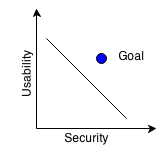
\includegraphics[scale=0.7]{pics/UsabilityVsSecurity.png}
    \end{center}
    \vspace{-20pt}
    \caption{Usability vs. Security}
    \vspace{-10pt}
  \end{wrapfigure}

  Authentication with text-based passwords are a common approach, but it is well known that users often choose weaker passwords because of the limitations of recalling text-based passwords. Graphical passwords came as an alternative solution for overcoming the limitations of text-based passwords, and was inspired by researchers that showed that the graphical memory of humans is particularly well-suited to remember graphical information\cite{DeAngeli}. The problem with many graphical password schemes is that they often promise improved password memorability and thus usability, while at the same time improving the security \cite{Biddle}. This is why it is important to understand both the usability and security aspects when looking at different password schemes in order to understand the trade off between different design choices.

\subsection{Usability and Memorability}

  {\color{red} \bf Finne forskning som evaluerer grafiske password på usability and memorability}

  An interesting question is what classes of graphical password users find memorable. Based on cognitive studies of visual information, Oorschot and Thorpe \cite{Thorpe} investigated the memorable password in the graphical password scheme DAS \cite{Jermyn}. They found that the were less or equal to the length of 8 on a 5$\times$5 grid. This results compared to textual passwords may offer greater security against dictionary attacks. 

  If the number of possible pictures in a graphical password scheme is large enuogh, and the diversity of the of picture based passwords can be captured, it seems reasonable to argue that memorable password space of a graphical password scheme will be higher than text-based password schemes, making graphical passwords offering better resistance to dictionary attacks.
  When the proposal for the graphical password scheme ``Deja Vu'' was proposed, they did a user study that showed that 90\% of all participants succeeded in the authentication tests using Deja Vu while only about 70\% succeeded using pass words and PINS \cite{DejaVu}. This is an example that users tends to have a higher success rate remembering graphical password, rather than text-based passwords. 

  One of the first graphical password schemes, ``DAS'' \cite{Jermyn}, offers a theoretical space that are compareable with text-based passwords, but results from research shows that users tends to draw symmetric images with few pen strokes, and often place their drawings in the center of the grid. The ``BDAS'' scheme \cite{BDAS} tried to avoid this by adding a additional background image, and the results showed that it reduced the amount of symmetry within password images, and supported the users to make longer passwords that were similarly memorable as for the ``DAS''. It remains still a problem that many of the reseach published on graphical passwords are preformed with a pen and paper approach, raising a question about the validy of the results. One problem may be that many graphical passwords are not implemented, but only a theoretical suggestions. It still remains a lot of reseach on graphical passwords in their inteded environment. 

  Davis \cite{Davis} did a comparison of the memorability between the graphical password scheme ``Face'' (a ligh version of the ``PassFaces'') and ``Story''. This results reported that users had more difficulty remembering Story password (success rate of 85\%), mostly of the errors was introduced because they had to remember the correct sequence of the images. 

  Wiedenbeck et al. \cite{Wiedenbeck1, Wiedenbeck2, Wiedenbeck3} conducted three lab-based user studies of the graphical password scheme ``PassPoint''. The results showed that the users needed an average time of 63 seconds in order to create their password, and an additional average time of 171 seconds in training time in order to remeber the password. The login time took an average time of 9 and 19 seconds. This highligts important reseach of usability and memorability of a graphical password scheme. Some of the factors that makes a password scheme to have hight usability is deciced by average creation time, time to remember the password, as well as time used in the login phase. 


    
\subsection{Security}

  In knowledge-based authentication, e.g. ``something you know'' we classify attacks into two general categories: guessing and capturing attacks. In a guessing attack the attackers are able to search through the entire password space, or either predict the users passwords patterns in order to avoid searching through the whole passwords space (often referred to as a dictionary attack). This is often associated with the entropy of the password, because the lower the entropy it will be easier to make a successful attack. When talking about capturing attacks, the attackers are able to directly obtain the passwords by observing the authentication process. One of the known capturing attacks on graphical passwords are shoulder surfing because of its graphical visualization.  

  Since a person needs to remember a password, it is normally to choose a password that are connected to you as a person in order to remember the password, causing the password to have bias. A bias can be explained as a prejudice in favor of or against one thing, person, or group compared with another, usually in a way that influence a person choice of action. Since psychological studies have recognized that the human brain have a superior memory for recognizing and recalling visual information, it support the statement that users are able to remember more complex graphical password form a larger password space than a alphanumeric password. Logically the attacker then have to build a bigger and more complex dictionary, thus spend more time to achieve the same success rate as for textual passwords. 

  The graphical password scheme DAS \cite{Jermyn} was evaluating the security of their password scheme. They highlighted that there are many factors that impacts the security of a password scheme, like the statement that the users do not use a uniform distribution of all possible passwords, using Klein's study \cite{UnixPasswords} as a argument. The fact that users do not pick passwords uniformly is not in itself a sufficient statement to make a guessing attack successful. They try to cover the possibility for a attacker making a successful attack by making their scheme complex, and the results showed that the generated passwords was significantly harder to crack in practice than textual passwords. The problem is that they used computer generated passwords that will not show actually password chosen by user. They did not analyze the security of the DAS including human factors and password biases that may could influence the practical password space. 

  {\bf \color{red} Her må jeg ha med flere eksempler på forskning som fokuserer på angrep}

  A clever attacker would narrow down the password space and prioritize guesses to pictures that people are likely to choose as a password. The images that are chosen are likely to be the pictures that users are likely to recall. 
  In order to understand how an attacker might take advantage of human password choices, psychological studies on humans visual memory are important to understand. 

\section{Psychology and Human Factors}

  \begin{wrapfigure}{r}{0.35\textwidth}
    \vspace{-20pt}
    \begin{center}
      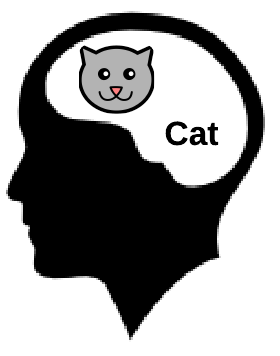
\includegraphics[scale=0.35]{pics/dualCoding.png}
    \end{center}
    \vspace{-20pt}
    \caption{Dual-Coding Theory}
    \vspace{-10pt}
  \end{wrapfigure}

  In many years, the field of psychology been a important in order to understand how humans interpret and remember different information. Psychology studies have recognized that the human brain have a superior memory for recognizing and recalling visual information rather than recognizing and recalling verbal or textual information \cite{DeAngeli}. One known theory is the ``dual-coding theory'' \cite{Biddle}, suggesting that verbal and non-verbal memory are processed and represented differently in humans mind. Text are verbal information that is represented symbolically, in contrast to non-verbal information like images that are mentally represented in a way that perceived concepts are assigned to a perceived meaning of what is directly observed. Both verbal and non-verbal information can be used when recalling information. For example, say a person have received stimulus of the concept ``cat'', both the image of a cat as well as the word ``cat''. When the person is asked to recall the concept ``cat'', the person can retrieve the image or the word individually, or both simultaneously. If the word ``cat'' is recalled, the image of the cat is not lost and can still be retrieved at a later point in time. The ability to code a stimulus in two different ways can increase humans ability to remember, in contrast to only code the stimulus in one way. In the background theory there are described three different categories of graphical passwords according to the memory task involved in remembering and entering the password, e.g. recall, recognition and cued-recall. 

  When it comes to humans and visual interpretation, studies supports the idea that people recall symmetric images better than asymmetric images \cite{Attneave, French}. A particular interesting observation is that mirror symmetry carries a special status i the human memory\cite{Wagemans}. A understanding of psychological studies on humans visual memory can help to build successfully attacks against graphical passwords. If an attacker can successfully use the symmetric properties of graphical password schemes, then the security may be significantly less than if all passwords were equivalent probable. 

  Humans do not only tend to choose symmetric passwords, but do also tend to be influenced by the graphical elements in a password scheme. A study on ``PassFace'' \cite{Davis} showed that there was a high bias in the password selection according to a users demography. When they analyzed how each gender choose their password, the most of the male and female participants chose female faces, and and 60-70\% of the user chose a model over a typical female/male. They also looked into the race of the faces, where the results showed that almost all of the participant chose their own race. 

  There is a lot of studies on password based on psychology and human factors, but the graphical passwords schemes being analyzed do not look at the background of the users. Humans are different in terms of their demographics, like gender, age and culture in their country. Analysis of people choices of graphical password based on users background have not been looked further into in published reseach as based on this state of the art research. 


  {\bf \color{red} Legge til mer forskning}

  {\bf \color{red} Studere papers fra Thorpe and Van Oorschot}
  

\section{Graphical Passwords and Mobile Devices}
  %Intro
  Users are not only dependent on remembering passwords across multiple web pages and systems, but do also need to remember passwords for our small mobile devices. The mobile phone have emerged as a good platform for graphical passwords because it is easier to input on touchscreen as a contrast to text-based passwords. Graphical passwords on mobile devices seems as a natural fit, as they often require direct manipulation of visual elements. In todays society we're addicted to our mobile devices in our every day life. Mobile devices are not just a communication tool for calling and texting, but also an important tool for every day tasks like doing our work, reading mail, pay our bills and keeping up with our social life. This trend makes our mobile devices vulnerable in terms of security. To avoid unwanted access, smartphones offers different locking mechanisms. The history of locking mechanisms was often a solution solely to prevent accidental use, while current mobile phones require protection in order to secure the potentially vast amount of private data that we keep on our smartphones. The situation of our rapidly use of mobile phones, as well as it well suited platform for graphical password, makes authentication on mobile devices an interesting field of study.

  When looking at mobile security it essential to be familiar with the magnitude of mobile phone usage. As of 2014, over 90\% of american adults owns a mobile phone, whereas 58\% of american adults owns a smartphone \cite{MobileUseage}. Another 34\% of the users used mostly their phone to go online instead of using other devices such as a desktop or laptop computer. This is numbers from USA, but it still provides insight into the how common mobile phones is today.

  % Awareness about the sensitivity of the data stored mobile phones
  As stated earlier, smartphone useres tends to store sensitive information on their phones, it is therefore important to understand the relationship between the use of security features and users risk percetions. One of the key security aspects on mobile phones that is important to understand is why people use or not use locking mechanisms on their smartphone. Engelman et al. \cite{Egelman} published a research paper in cooperation with Google on peoples smartphone locking behavior and attitudes towards security of their smartphone data. They observed a strong correlation between use of security features and risk perceptions. They reported that 33\% of the smartphone users were thinking about the locking mechanisms as too much of a hassle, while 26\% of the useres didnt think that someone would care about the information stored on their phone.  Other reported results have covered that the 46.8\% of the participants agreed or fully agreed that unlocking their phone can be annoying, but at the same time 95.5\% of the somewhat or fully agreed that they liked the idea that their phone was protected \cite{habits3}. A study reported that 29\% did not lock their smartphones \cite{MobileUseage}, while another reseach stated that among 35\% of mobile users dont lock their phone \cite{Bruggen}. The number may vary becuase of the background and experiences with security , but the number still remains quite high. This highlights that the users wants to be secure, but there might be a trade-off between the time used to unlock the smartphone vs the security risk. 

  % The time used on unlocking the phone
  In terms of security it is interesting to look at the use of mobile devices and look at the locking habits among users on mobile devices. It is known that services that are rapidly used have weaker password because of the overhead the user needs to spend on typing their password. In 2014 a group of researchers published a field study of smartphone (un)locking behavior \cite{habits3}. Some of the problems with smartphone users tends to be their rapidly use of their phone. When the device are rabidly use, it results in a lot of time unlocking their phone between every use. In the study they found that there was a significant overhead in the time used of unlocking their phone, where the users participated in the field study used 2.9\% (9\% in the worst case) of their time unlocking their smartphone. 

  It is stated that a lot of useres use their smartphones to perform tasks that involve use and storage of sensitive data. Smartphones in use today do not require their users to have a locking mechanism on their smartphone. It is well known that users tends to choose to easiest way out and may result in the choice of not having any locking mechanism at all. Based on the result of the overhead in time used on unlocking their phone, a result may be to take the easiest way out by ignoring the vulnerability of not using a locking mechanism at all. It have been discovered that over 40\% of the users only used a basic ``slide-to-unlock'' mechanism on their smartphone, as well as over 16\% didn't use any locking mechanisms at all \cite{habits3}. This highlights a major bad habit among mobile users. What happens if your mobile is stolen? A loss of a mobile phone is not just the cost for replacing the phone, but also a loss of sensitive data. If the phone is found by the worong persons, the sensitive data on the phone may be lost and used for unintended purposes. A 2012 report from Pew Internet estimated that nearly a third of cell phone users have had their device stolen or lost \cite{StolenLost}. It is interesting to comparing peoples locking behavior towards phones that are stolen or lost. The same report also reported that 12\% of cell owners say that another person have accessed their phone, making the owners feel that their privacy have been exposed to the public.

  Beside loosing a physical device, whar concequences are users exposed to? One point of attack is a persons email. If you can grant access to someones email, you probably can get access to a lot more. In a study reported that all of their interview participants had their email account automatically loged in, as well as 31\% of them did not use any locking mechanism at all \cite{Egelman}. The same reseach group investigated how much information you could gain from getting access to a persons email account. The results showed that both users with or without locking mechanisms found sensitive information in their email account like SSN, Bank Account Number, Email Password and Home Address.

  One of the popular password schemes on mobile phones are the Android Unlock pattern. It is a graphical password that have been shown to have biases when the password are user-chosen. A research group did a large-scale user study on the Android Unlock Patterns in order to quantify its security \cite{Uellenbeck}. They analyses the biases introduced in the pattern making process and added changes to the scheme in order to avoid the known biases in the password scheme. The researchers found that there is a high bias in the pattern selection process, e.g. the upper left corner and three-point long straight lines are very typical selection strategies. If the patterns was uniformly chosen, the probability of starting in the top-left corner should be 11\%, but are instead close to 44\%. Another interesting result is the memorable password space used, where about 10\% of all users use less than 190 patterns, while less than 300 patterns capture around 50\% of the whole test population. This shows that a empirical password space are not a representative number when quantifying the security of a password, but we should look at the memorable password space, e.g. password that actually are used and memorable for the useres. The Android Unlock Patterns are a password scheme used on mobile devices. It is important to understand the difference of a password scheme used on a desktop vs. mobile device.

  The way that the mobile phone is held, the size of the screen may also impact the way that people write their passwords, but this may need further research to answer.

  